\documentclass{beamer}
%
% Choose how your presentation looks.
%
% For more themes, color themes and font themes, see:
% http://deic.uab.es/~iblanes/beamer_gallery/index_by_theme.html
%
\mode<presentation>
{
  \usetheme{default}      % or try Darmstadt, Madrid, Warsaw, ...
  \usecolortheme{default} % or try albatross, beaver, crane, ...
  \usefonttheme{default}  % or try serif, structurebold, ...
  \setbeamertemplate{navigation symbols}{}
  \setbeamertemplate{caption}[numbered]
} 

\usepackage[english]{babel}
\usepackage[utf8x]{inputenc}
\usepackage{booktabs}
\title[Your Short Title]{Letter Classification}
\author{Matt Oehler and Jackson Curtis}
\institute{Stat 536}
\date{\today}

\begin{document}

\begin{frame}
  \titlepage
\end{frame}

% Uncomment these lines for an automatically generated outline.
%\begin{frame}{Outline}
%  \tableofcontents
%\end{frame}

\section{Introduction}

\begin{frame}{Intro To Support Vector Machines}
Support vector machines define dividing hyperplanes 
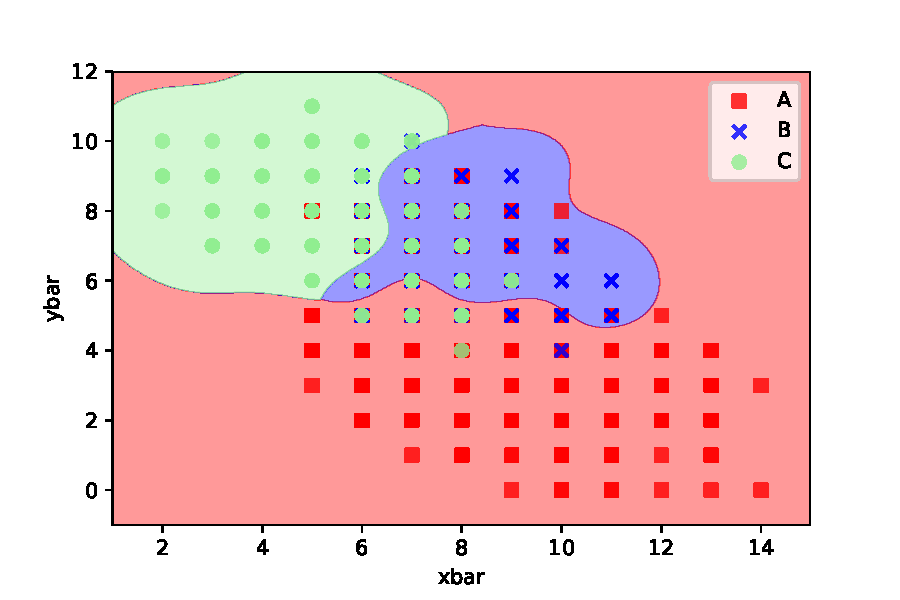
\includegraphics[scale=.4]{DemoSVM.pdf}
\end{frame}

\begin{frame}{Overall Accuracy}
\begin{table}
\centering
\begin{tabular}{lr}
Method & Out of Sample Accuracy \\
\hline
Random Forest & 96.70\% \\
Support Vector Machine & 97.77\% \\
\end{tabular}
\caption{SVMs slightly outperform Random Forests with 1000 trees and max 3 features}
\end{table}
\end{frame}

\begin{frame}{Letter Ranking}
\begin{table}

\centering
\begin{tabular}{rl}
\toprule
  Accuracy & Letter \\
\midrule
    0.9987 &      A \\
    0.9947 &      S \\
    0.9926 &      U \\
    0.9920 &      W \\
    0.9911 &      Y \\
    0.9905 &      Z \\
    0.9886 &      X \\
    0.9885 &      Q \\
    0.9874 &      M \\
    0.9862 &      T \\
    0.9842 &      L \\
    0.9823 &      C \\
    0.9819 &      G \\
    \bottomrule
\end{tabular}
    \begin{tabular}{rl}
\toprule
   &  \\
\midrule
    0.9801 &      O \\
    0.9776 &      D \\
    0.9766 &      E \\
    0.9764 &      V \\
    0.9745 &      N \\
    0.9726 &      B \\
    0.9652 &      F \\
    0.9639 &      J \\
    0.9621 &      K \\
    0.9617 &      R \\
    0.9616 &      I \\
    0.9614 &      P \\
    0.9319 &      H \\
\bottomrule
\end{tabular}

\caption{Ranking of which letters are easiest to predict}
\end{table}

\end{frame}





\begin{frame}{Future Work}
\itemize
\item Results could be improved be ensembling several different approaches.
\item Added features would probably help SVM (does well in high dimensions)
\item At the extreme, neural nets could be used on pixel by pixel information
\end{frame}

\subsection{Mathematics}

\begin{frame}{Readable Mathematics}

Let $X_1, X_2, \ldots, X_n$ be a sequence of independent and identically distributed random variables with $\text{E}[X_i] = \mu$ and $\text{Var}[X_i] = \sigma^2 < \infty$, and let
$$S_n = \frac{X_1 + X_2 + \cdots + X_n}{n}
      = \frac{1}{n}\sum_{i}^{n} X_i$$
denote their mean. Then as $n$ approaches infinity, the random variables $\sqrt{n}(S_n - \mu)$ converge in distribution to a normal $\mathcal{N}(0, \sigma^2)$.

\end{frame}

\end{document}
